\documentclass[../../deliverable-two.tex]{subfiles}
\graphicspath{
  {\subfix{../../../api/}}
}

\begin{document}

\subsection{Komunikacja użytkownika z systemem - REST API}

Komunikacja aplikacji klienckiej oraz panelu administratora z systemem - nadzorcą - rozwiązana jest za pomocą REST API\footnote{\href{https://restfulapi.net/}{Opis REST API}}. Wiadomości wysyłane są za pomocą protokołu HTTPS\footnote{\href{https://datatracker.ietf.org/doc/html/rfc2818}{Specyfikacja protokołu HTTP Over TLS}}, który zapewnia ich szyfrowanie. W tym celu wymagane jest, aby na adres, pod którym udostępniony będzie system, wystawiony był odpowiedni certyfikat\footnote{\href{https://protonmail.com/blog/tls-ssl-certificate/}{Opis certyfikatu TLS/SSL}}, gwarantujący jego tożsamość. Podczas tworzenia systemu i testów możliwe jest użycie sztucznego, własnoręcznie podpisanego certyfikatu\footnote{\href{https://aboutssl.org/what-is-self-sign-certificate/}{Opis własnoręcznie podpisanego certyfikatu TLS/SSL}}.

Całość specyfikacji API umieszczona jest w osobnym pliku. Poniżej znajduje się zestawienie oraz krótki opis endpointów.

\begin{figure}[H]
    \centering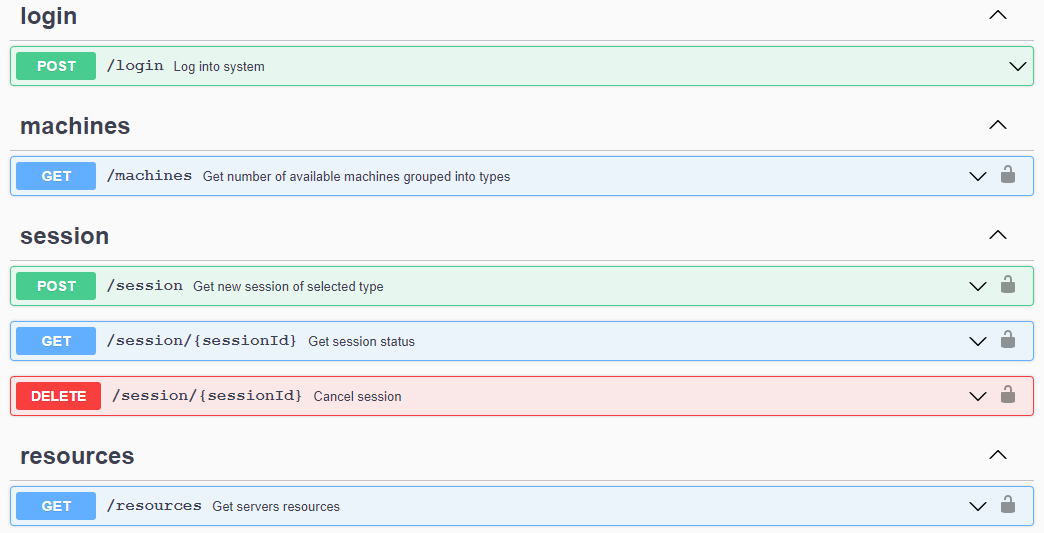
\includegraphics[width=0.9\textwidth]{endpoints.png}
    \caption{Endpointy API}
\end{figure}

\begin{itemize}
    \item Login - służy do logowania do systemu; współdzielony przez aplikację kliencką oraz panel administracyjny. Poprawne zalogowanie zwraca token do dalszej autoryzacji.
    \item Machines - służy do pobierania przez aplikację informacji o typach i ilości dostępnych maszyn. Utworzenie sesji jest możliwe poprzez \texttt{POST} z typem maszyny. W odpowiedzi użytkownik dostaje częściowo wypełniony obiekt sesji zawierający id umożliwiające dalsze zapytania. \texttt{GET} zwraca obiekt sesji z aktualnym stanem. Jeżeli sesja jest gotowa, to zawiera on też adres, z którym należy nawiązać połączenie RDP. Ten endpoint, oraz wszystkie następne wymagają autoryzacji poprzez umieszczenie tokenu otrzymanego podczas logowania w odpowiednim nagłówku wiadomości, oraz dostępne są tylko dla użytkownika.
    \item Session - pozwala na wysłanie prośby o uzyskanie sesji, pobranie stanu sesji oraz jej anulowanie.
    \item Resources - udostępnia informację o zasobach działających serwerów wirtualizacji. Dostępny jedynie dla administratora.
\end{itemize}

\subsection{Komunikacja wewnątrz systemu - broker wiadomości}

Do komunikacji wewnątrz systemowej użyty jest broker wiadomości RabbitMQ. Umożliwia on wysyłanie asynchronicznych wiadomości do wielu odbiorców jednocześnie. Dzięki temu żaden z modułów nie musi znać dokładnej liczby oraz adresów modułów, z którymi chce się komunikować.
Wewnątrz systemu działa dwóch brokerów wiadomości. Jeden, główny, służy do komunikacji pomiędzy nadzorcami i serwerami wirtualizacji. Obsługuje on kanał, którego nadawcami są nadzorcy, a odbiorcami serwery wirtualizacji oraz kanał z odwrotną komunikacją. Wiadomości wysyłane przez nadzorcę do wszystkich serwerów wysyłane są pierwszą z kolejek,

\end{document}